\section{Our Mining Framework for Ethereum}\label{sec/mining-ethereum-algorithm} 

We start this section with a high-level overview of our algorithm and then provide the details of each step. The fundamental idea behind our approach is a simple observation: in real-world instances of the problem, each transaction interacts with only a few other transactions, which we call its neighborhood. Thus, when forming a block, we do not need to search over all possible permutations of transactions, but can instead find rules that encode the gas usage of each transaction based on the portion of its neighborhood that precedes it in the block.

\paragraph{Overview} Our approach consists of the following steps:
\begin{enumerate}
	\item \emph{Sampling and Testing.} We start by sampling random permutations of the transactions available in our $\pool$ and executing them, keeping track of the amount of gas used by each transaction in each sample permutation.
	\item \emph{Neighborhood Estimation.} For each transaction $\tx,$ we identify a neighborhood, i.e.~a set $\nbhd(\tx)$ of transactions whose inclusion before $\tx$ has the potential to change the amount of gas consumed by $\tx.$ To estimate each transaction's neighborhood, we rely on a decision tree generated from our samples.
	\item \emph{Extracting Gas Usage Rules.} Using the neighborhoods and samples, we extract gas usage rules.  We define a simple grammar that can encode rules such as ``if $\tx_1$ appears before $\tx_2$ which in turn appears before $\tx_3,$ then $\tx_3$ will have a gas usage of $g$'' for $\tx_1, \tx_2 \in \nbhd(\tx_3).$ We show that such rules can be mined from our samples, using a different decision tree.
	\item \emph{Translating Gas Usage Rules to ILP.} Our goal is to obtain a block that orders a subset of transactions in a manner that maximizes the total tip earned by the miner. To do this, we have to choose which rules from the previous step to follow, i.e. which local orderings to include, but cannot choose rules that require conflicting orders on the transactions. Our algorithm translates this problem to integer linear programming (ILP).
	\item \emph{Solving the ILP.} Finally, we call an external off-the-shelf ILP-solver to handle the ILP instance generated in the previous step. This yields the desired block. 
\end{enumerate}



\paragraph{Step (1): Sampling and Testing}
The input to our algorithm is the initial world state $s_0$ and a set $\pool = \{ \tx_1, \tx_2, \ldots, \tx_n \}$ of valid transactions which are not yet added to the blockchain. In this step, we randomly and uniformly generate several permutations $\Pi = \{\pi_1, \pi_2, \ldots, \pi_k\}$ of our $\pool.$ The number of samples, $k,$ is a user-defined parameter. Note that the $\pi_i$'s are not necessarily valid blocks as they might exceed the block gas limit.

% Question: Does this mean that we removed faulty transactions for orders?
We need to perform some simple housekeeping at this point. Recall that transactions originating from the same account should appear in the order of their nonces. We say a transaction $\tx$ is an $a$-transaction if it originates from an account with address $a.$ For every $i$ and $a,$ we sort all the $a$-transactions in $\pi_i$ by their nonce, thus ensuring that every sample $\pi_i$ respects nonce orders. If there are several $a$-transactions with the same nonce in $\pi_i$, we only keep the first and remove the rest. Thus, $\pi_i$ might end up containing only a subset of the transactions in $\pool.$

We then execute every sample $\pi_i$ starting from the initial world state $s_0$ and keep track of the amount of gas used by each transaction $\tx_j$ in the execution of $\pi_i.$ We denote this by $\gas(\pi_i, \tx_j).$


\paragraph{Example} Suppose we have 6 transactions in our pool and the tip value set by the users is $t[\tx_1, \tx_2, \tx_3,  \tx_4,  \tx_5,  \tx_6] = [24, 9, 5, 29, 24, 2],$ i.e.~$\tx_1$ pays a tip of $24$ for each consumed unit of gas, $\tx_2$ pays $9,$ etc. We generate $k=10$ random permutations $\pi_1, \ldots, \pi_{10}$ of the pool, execute them, and keep track of the gas used by each transaction in each sample.  See Figure~\ref{fig:mining-ethereum-fuzzing}.


\paragraph{Step (2): Neighborhood Estimation} In this step, we consider each transaction $\tx_i \in \pool$ separately and our goal is to identify a neighborhood for it, i.e.~a set of transactions $\nbhd(\tx_i) \subseteq \pool$ whose inclusion before $\tx_i$ can potentially change the amount of gas consumed by $\tx_i.$ We observe that the transactions usually exhibit only a few different possible gas usage values. Thus, we can use the amount of gas used by $\tx_i$ as a label in a classification problem. We introduce one binary attribute for each $\tx_j,$ which is set to $1$ if $\tx_j$  precedes $\tx_i$ in the sample permutation. We then generate a decision tree. At each node of the tree, we choose the best possible attribute to branch on, based on the Gini impurity metric \cite[Chapter 4.6]{breimanClassification1984}. After generating the decision tree, if the attribute corresponding to $\tx_j$ appears in one of the decisions, we add $\tx_j$ to the neighborhood $\nbhd(\tx_i).$

\paragraph{Example} Consider the samples of the previous example (Figure~\ref{fig:mining-ethereum-fuzzing}). In this step, our algorithm finds a neighborhood for every transaction. Let us consider $\tx_3.$ We can encode each permutation $\pi_i$ as a vector $v_i$ such that $v_i[j] = 1$ if $\tx_j$ precedes $\tx_3$ in $\pi_i$ and $v_i[j]=0$ otherwise. The label associated with $v_i$ is the gas usage of $\tx_3$ in the execution of $\pi_i.$ In this case, there are only two possible labels: $2$ and $4$. See Figure~\ref{fig:mining-ethereum-dectree} (left). When we generate a decision tree, shown in Figure~\ref{fig:mining-ethereum-dectree} (right), it only looks at the attribute corresponding to $\tx_2.$ Hence, we set $\nbhd(\tx_3) = \{\tx_2\}.$ In other words, at least in our samples, the gas usage of $\tx_3$ is only dependent on whether $\tx_2$ precedes it. This is shown in Figure~\ref{fig:mining-ethereum-nei}.

\clearpage

\begin{figure}[!p]
\centering
\begin{tikzpicture}[scale=1.5, transform shape, every node/.style={font=\small}]
	% Permutation deabcf: 554 gas: [2, 10, 6, 8, 4, 10] (sum: 40) fees: [58, 240, 144, 72, 20, 20] (sum: 554)
	\def\row{0}
	\def\col{0}
	\txheader{(0 + \col)}{\row}
	\txd   {2}   {58 } {(1 + \col)}{\row}
	\txe  {10}  {240 } {(2 + \col)}{\row}
	\txa   {6}  {144 } {(3 + \col)}{\row}
	\txb   {8}   {72 } {(4 + \col)}{\row}
	\txc   {4}   {20 } {(5 + \col)}{\row}
	\txf  {10}   {20 } {(6 + \col)}{\row}
	\txres{1}{40}  {554 } {(7 + \col)}{\row}
	
	% Permutation bdacef: 410 gas: [8, 2, 8, 4, 2, 10] (sum: 34) fees: [72, 58, 192, 20, 48, 20] (sum: 410)
	\def\row{0}
	\def\col{7.5}
	% \txheader{(0 + \col)}{\row}
	\txb{ 8}{ 72 }{(1 + \col)}{\row}
	\txd{ 2}{ 58 }{(2 + \col)}{\row}
	\txa{ 8}{192 }{(3 + \col)}{\row}
	\txc{ 4}{ 20 }{(4 + \col)}{\row}
	\txe{ 2}{ 48 }{(5 + \col)}{\row}
	\txf{10}{ 20 }{(6 + \col)}{\row}
	\txres{2}{34}{410 }{(7 + \col)}{\row}
\end{tikzpicture}

\begin{tikzpicture}[scale=1.5, transform shape, every node/.style={font=\small}]
	% Permutation bcfaed: 506 gas: [8, 4, 10, 10, 4, 2] (sum: 38) fees: [72, 20, 20, 240, 96, 58] (sum: 506)
	\def\row{0}
	\def\col{0}
	\txheader{(0 + \col)}{\row}
	\txb{8}{72 }{(1 + \col)}{\row}
	\txc{4}{20 }{(2 + \col)}{\row}
	\txf{10}{20 }{(3 + \col)}{\row}
	\txa{10}{240 }{(4 + \col)}{\row}
	\txe{4}{96 }{(5 + \col)}{\row}
	\txd{2}{58 }{(6 + \col)}{\row}
	\txres{3}{38}{506 }{(7 + \col)}{\row}
	
	
	% Permutation dacfeb: 601 gas: [2, 8, 2, 10, 10, 9] (sum: 41) fees: [58, 192, 10, 20, 240, 81] (sum: 601)
	\def\row{0}
	\def\col{7.5}
	% \txheader{(0 + \col)}{\row}
	\txd{2}{58 }{(1 + \col)}{\row}
	\txa{8}{192 }{(2 + \col)}{\row}
	\txc{2}{10 }{(3 + \col)}{\row}
	\txf{10}{20 }{(4 + \col)}{\row}
	\txe{10}{240 }{(5 + \col)}{\row}
	\txb{9}{81 }{(6 + \col)}{\row}
	\txres{4}{41}{601 }{(7 + \col)}{\row}
\end{tikzpicture}

\begin{tikzpicture}[scale=1.5, transform shape, every node/.style={font=\small}]
	% Permutation dfeabc: 553 gas: [2, 5, 10, 6, 9, 4] (sum: 36) fees: [58, 10, 240, 144, 81, 20] (sum: 553)
	\def\row{0}
	\def\col{0}
	\txheader{(0 + \col)}{\row}
	\txd{2}{58 }{(1 + \col)}{\row}
	\txf{5}{10 }{(2 + \col)}{\row}
	\txe{10}{240 }{(3 + \col)}{\row}
	\txa{6}{144 }{(4 + \col)}{\row}
	\txb{9}{81 }{(5 + \col)}{\row}
	\txc{4}{20 }{(6 + \col)}{\row}
	\txres{5}{36}{553 }{(7 + \col)}{\row}
	
	% Permutation fdcbae: 591 gas: [5, 2, 2, 9, 8, 10] (sum: 36) fees: [10, 58, 10, 81, 192, 240] (sum: 591)
	
	\def\row{0}
	\def\col{7.5}
	% \txheader{(0 + \col)}{\row}
	\txf{5}{10 }{(1 + \col)}{\row}
	\txd{2}{58 }{(2 + \col)}{\row}
	\txc{2}{10 }{(3 + \col)}{\row}
	\txb{9}{81 }{(4 + \col)}{\row}
	\txa{8}{192 }{(5 + \col)}{\row}
	\txe{10}{240 }{(6 + \col)}{\row}
	\txres{6}{36}{591 }{(7 + \col)}{\row}
\end{tikzpicture}

\begin{tikzpicture}[scale=1.5, transform shape, every node/.style={font=\small}]
	% Permutation efacdb: 447 gas: [10, 5, 2, 2, 2, 9] (sum: 30) fees: [240, 10, 48, 10, 58, 81] (sum: 447)
	\def\row{0}
	\def\col{0}
	\txheader{(0 + \col)}{\row}
	\txheader{(0 + \col)}{\row}
	\txe{10}{240 }{(1 + \col)}{\row}
	\txf{5}{10 }{(2 + \col)}{\row}
	\txa{2}{48 }{(3 + \col)}{\row}
	\txc{2}{10 }{(4 + \col)}{\row}
	\txd{2}{58 }{(5 + \col)}{\row}
	\txb{9}{81 }{(6 + \col)}{\row}
	\txres{7}{30}{447 }{(7 + \col)}{\row}  
	
	
	% Permutation adecbf: 640 gas: [10, 2, 10, 2, 8, 10] (sum: 42) fees: [240, 58, 240, 10, 72, 20] (sum: 640)
	\def\row{0}
	\def\col{7.5}
	% \txheader{(0 + \col)}{\row}
	\txa{10}{240 }{(1 + \col)}{\row}
	\txd{2}{58 }{(2 + \col)}{\row}
	\txe{10}{240 }{(3 + \col)}{\row}
	\txc{2}{10 }{(4 + \col)}{\row}
	\txb{8}{72 }{(5 + \col)}{\row}
	\txf{10}{20 }{(6 + \col)}{\row}
	\txres{8}{42}{640 }{(7 + \col)}{\row}
\end{tikzpicture}

\begin{tikzpicture}[scale=1.5, transform shape, every node/.style={font=\small}]
	% Permutation cfbead: 313 gas: [2, 10, 9, 4, 2, 2] (sum: 29) fees: [10, 20, 81, 96, 48, 58] (sum: 313)
	\def\row{0}
	\def\col{0}
	\txheader{(0 + \col)}{\row}
	\txc{2}{10 }{(1 + \col)}{\row}
	\txf{10}{20 }{(2 + \col)}{\row}
	\txb{9}{81 }{(3 + \col)}{\row}
	\txe{4}{96 }{(4 + \col)}{\row}
	\txa{2}{48 }{(5 + \col)}{\row}
	\txd{2}{58 }{(6 + \col)}{\row}
	\txres{9}{29}{313 }{(7 + \col)}{\row}
	
	% Permutation bacedf: 506 gas: [8, 10, 4, 4, 2, 10] (sum: 38) fees: [72, 240, 20, 96, 58, 20] (sum: 506)
	\def\row{0}
	\def\col{7.5}
	% \txheader{(0 + \col)}{\row}
	\txb{8}{72 }{(1 + \col)}{\row}
	\txa{10}{240 }{(2 + \col)}{\row}
	\txc{4}{20 }{(3 + \col)}{\row}
	\txe{4}{96 }{(4 + \col)}{\row}
	\txd{2}{58 }{(5 + \col)}{\row}
	\txf{10}{20 }{(6 + \col)}{\row}
	\txres{10}{38}{506 }{(7 + \col)}{\row}
\end{tikzpicture}
\caption{An example execution of $10$ samples of a pool of $6$ transactions, profiling the gas usage and tip revenue obtained from each transaction.} 
\label{fig:mining-ethereum-fuzzing}
\end{figure}

\begin{figure}[!p]
\centering
\begin{tikzpicture}[scale=1.5, transform shape, every node/.style={font=\small}]
	% Permutation deabcf: 554 gas: [2, 10, 6, 8, 4, 10] (sum: 40) fees: [58, 240, 144, 72, 20, 20] (sum: 554)
	\def\row{0}
	\def\col{0}
	\txheader{(0 + \col)}{\row}
	\txdOff   {2}   {58 } {(1 + \col)}{\row}
	\txeOff  {10}  {240 } {(2 + \col)}{\row}
	\txaOff   {6}  {144 } {(3 + \col)}{\row}
	\txbN   {8}   {72 } {(4 + \col)}{\row}
	\txcOn   {4}   {20 } {(5 + \col)}{\row}
	\txfOff  {10}   {20 } {(6 + \col)}{\row}
	
	% Permutation bdacef: 410 gas: [8, 2, 8, 4, 2, 10] (sum: 34) fees: [72, 58, 192, 20, 48, 20] (sum: 410)
	\def\row{0}
	\def\col{7}
	% \txheader{(0 + \col)}{\row}
	\txbN{ 8}{ 72 }{(1 + \col)}{\row}
	\txdOff{ 2}{ 58 }{(2 + \col)}{\row}
	\txaOff{ 8}{192 }{(3 + \col)}{\row}
	\txcOn{ 4}{ 20 }{(4 + \col)}{\row}
	\txeOff{ 2}{ 48 }{(5 + \col)}{\row}
	\txfOff{10}{ 20 }{(6 + \col)}{\row}
\end{tikzpicture}

\begin{tikzpicture}[scale=1.5, transform shape, every node/.style={font=\small}]
	% Permutation bcfaed: 506 gas: [8, 4, 10, 10, 4, 2] (sum: 38) fees: [72, 20, 20, 240, 96, 58] (sum: 506)
	\def\row{0}
	\def\col{0}
	\txheader{(0 + \col)}{\row}
	\txbN{8}{72 }{(1 + \col)}{\row}
	\txcOn{4}{20 }{(2 + \col)}{\row}
	\txfOff{10}{20 }{(3 + \col)}{\row}
	\txaOff{10}{240 }{(4 + \col)}{\row}
	\txeOff{4}{96 }{(5 + \col)}{\row}
	\txdOff{2}{58 }{(6 + \col)}{\row}
	
	
	% Permutation dacfeb: 601 gas: [2, 8, 2, 10, 10, 9] (sum: 41) fees: [58, 192, 10, 20, 240, 81] (sum: 601)
	\def\row{0}
	\def\col{7}
	% \txheader{(0 + \col)}{\row}
	\txdOff{2}{58 }{(1 + \col)}{\row}
	\txaOff{8}{192 }{(2 + \col)}{\row}
	\txcOn{2}{10 }{(3 + \col)}{\row}
	\txfOff{10}{20 }{(4 + \col)}{\row}
	\txeOff{10}{240 }{(5 + \col)}{\row}
	\txbN{9}{81 }{(6 + \col)}{\row}
\end{tikzpicture}

\begin{tikzpicture}[scale=1.5, transform shape, every node/.style={font=\small}]
	% Permutation dfeabc: 553 gas: [2, 5, 10, 6, 9, 4] (sum: 36) fees: [58, 10, 240, 144, 81, 20] (sum: 553)
	\def\row{0}
	\def\col{0}
	\txheader{(0 + \col)}{\row}
	\txdOff{2}{58 }{(1 + \col)}{\row}
	\txfOff{5}{10 }{(2 + \col)}{\row}
	\txeOff{10}{240 }{(3 + \col)}{\row}
	\txaOff{6}{144 }{(4 + \col)}{\row}
	\txbN{9}{81 }{(5 + \col)}{\row}
	\txcOn{4}{20 }{(6 + \col)}{\row}
	
	% Permutation fdcbae: 591 gas: [5, 2, 2, 9, 8, 10] (sum: 36) fees: [10, 58, 10, 81, 192, 240] (sum: 591)
	
	\def\row{0}
	\def\col{7}
	% \txheader{(0 + \col)}{\row}
	\txfOff{5}{10 }{(1 + \col)}{\row}
	\txdOff{2}{58 }{(2 + \col)}{\row}
	\txcOn{2}{10 }{(3 + \col)}{\row}
	\txbN{9}{81 }{(4 + \col)}{\row}
	\txaOff{8}{192 }{(5 + \col)}{\row}
	\txeOff{10}{240 }{(6 + \col)}{\row}
\end{tikzpicture}

\begin{tikzpicture}[scale=1.5, transform shape, every node/.style={font=\small}]
	% Permutation efacdb: 447 gas: [10, 5, 2, 2, 2, 9] (sum: 30) fees: [240, 10, 48, 10, 58, 81] (sum: 447)
	\def\row{0}
	\def\col{0}
	\txheader{(0 + \col)}{\row}
	\txheader{(0 + \col)}{\row}
	\txeOff{10}{240 }{(1 + \col)}{\row}
	\txfOff{5}{10 }{(2 + \col)}{\row}
	\txaOff{2}{48 }{(3 + \col)}{\row}
	\txcOn{2}{10 }{(4 + \col)}{\row}
	\txdOff{2}{58 }{(5 + \col)}{\row}
	\txbN{9}{81 }{(6 + \col)}{\row}
	
	
	% Permutation adecbf: 640 gas: [10, 2, 10, 2, 8, 10] (sum: 42) fees: [240, 58, 240, 10, 72, 20] (sum: 640)
	\def\row{0}
	\def\col{7}
	% \txheader{(0 + \col)}{\row}
	\txaOff{10}{240 }{(1 + \col)}{\row}
	\txdOff{2}{58 }{(2 + \col)}{\row}
	\txeOff{10}{240 }{(3 + \col)}{\row}
	\txcOn{2}{10 }{(4 + \col)}{\row}
	\txbN{8}{72 }{(5 + \col)}{\row}
	\txfOff{10}{20 }{(6 + \col)}{\row}
\end{tikzpicture}

\begin{tikzpicture}[scale=1.5, transform shape, every node/.style={font=\small}]
	% Permutation cfbead: 313 gas: [2, 10, 9, 4, 2, 2] (sum: 29) fees: [10, 20, 81, 96, 48, 58] (sum: 313)
	\def\row{0}
	\def\col{0}
	\txheader{(0 + \col)}{\row}
	\txcOn{2}{10 }{(1 + \col)}{\row}
	\txfOff{10}{20 }{(2 + \col)}{\row}
	\txbN{9}{81 }{(3 + \col)}{\row}
	\txeOff{4}{96 }{(4 + \col)}{\row}
	\txaOff{2}{48 }{(5 + \col)}{\row}
	\txdOff{2}{58 }{(6 + \col)}{\row}
	
	% Permutation bacedf: 506 gas: [8, 10, 4, 4, 2, 10] (sum: 38) fees: [72, 240, 20, 96, 58, 20] (sum: 506)
	\def\row{0}
	\def\col{7}
	% \txheader{(0 + \col)}{\row}
	\txbN{8}{72 }{(1 + \col)}{\row}
	\txaOff{10}{240 }{(2 + \col)}{\row}
	\txcOn{4}{20 }{(3 + \col)}{\row}
	\txeOff{4}{20 }{(4 + \col)}{\row}
	\txdOff{2}{58 }{(5 + \col)}{\row}
	\txfOff{10}{20 }{(6 + \col)}{\row}
\end{tikzpicture}
\caption{The gas usage of $\tx_3$ only depends on whether $\tx_2$ preceded it in the sample permutation.}
\label{fig:mining-ethereum-nei}

\end{figure}

\clearpage


\begin{figure}[h]
\centering
\begin{minipage}{0.48\textwidth}
\centering
\begin{tabular}{|c|c|c|}
    \hline
    Sample ($\pi_i$) & Encoding ($v_i$) & Label ($\gamma_3$)\\ \hline\hline
    $\pi_1$ & $[1, 1, 0, 1, 1, 0]$ &  $4$ \\
    $\pi_2$ & $[1, 1, 0, 1, 0, 0]$ &  $4$ \\
    $\pi_3$ & $[0, 1, 0, 0, 0, 0]$ &  $4$ \\
    $\pi_4$ & $[1, 0, 0, 1, 0, 0]$ &  $2$ \\
    $\pi_5$ & $[1, 1, 0, 1, 1, 1]$ &  $4$ \\
    $\pi_6$ & $[0, 0, 0, 1, 0, 1]$ &  $2$ \\
    $\pi_7$ & $[1, 0, 0, 0, 1, 1]$ &  $2$ \\
    $\pi_8$ & $[1, 0, 0, 1, 1, 0]$ &  $2$ \\
    $\pi_9$ & $[0, 0, 0, 0, 0, 0]$ & $2$ \\
    $\pi_{10}$ & $[1, 1, 0, 0, 0, 0]$ &  $4$ \\ 
    \hline
\end{tabular}
\end{minipage}
\hfill
\begin{minipage}{0.48\textwidth}
\centering
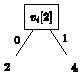
\includegraphics[scale=2.5]{chapters/mining/mining-ethereum-figures/dectree.pdf}
\end{minipage}
\caption{The classification problem is based on the gas used by $\tx_3$ (left) and the resulting decision tree (right).} 
\label{fig:mining-ethereum-dectree}
\end{figure}